\section{工具证据控制智能体工作流}

任务接口暴露可编辑的内核、公开测试、目标器件和预算，同时隐藏秘密测试和冻结
参考。控制器在单个运行状态中记录每个候选方案、门限、度量指标、令牌和积分。

\VCL{} 依次运行七个门限：接口（Interface）、\CSim、\Synth、频率（Frequency）、
容量（Capacity）、所需 \CoSim{} 和指标完备性（Metric completeness）。频率门
强制 100\,MHz，容量门强制 U55C 限制，\CoSim{} 仅在任务需要时适用。定义
有效性 $V(c)=\prod_i G_i$，其中 $G_i\in\{0,1\}$ 为各适用门的判定结果；不适用
的门贡献为 $1$。令 $b$ 为已验证备选方案。提升规则为
$P(c)=V(c)\land[Q_{\mathrm{HW}}(c)>Q_{\mathrm{HW}}(b)]$。预算准入为所有必需
门保留积分；门失败或预算不足则保留 $b$。QoR-RAG 提供版本兼容的规则和测量
结果。失败反思将诊断信息转化为下一轮约束，无需额外 LLM 请求。重复候选方案
和重复失败触发停止。

图~\ref{fig:vcl} 总结该回路。三次实验共记录 \CandidateEventCount{} 次候选
检查、\CandidateInterfaceRejectCount{} 次接口拒绝、\CandidateSynthGateCount{}
次综合门和 \CandidateCosimGateCount{} 次 \CoSim{} 门，确立了契约执行，但并未
隔离各机制的效果。

\begin{figure*}[t]
  \centering
  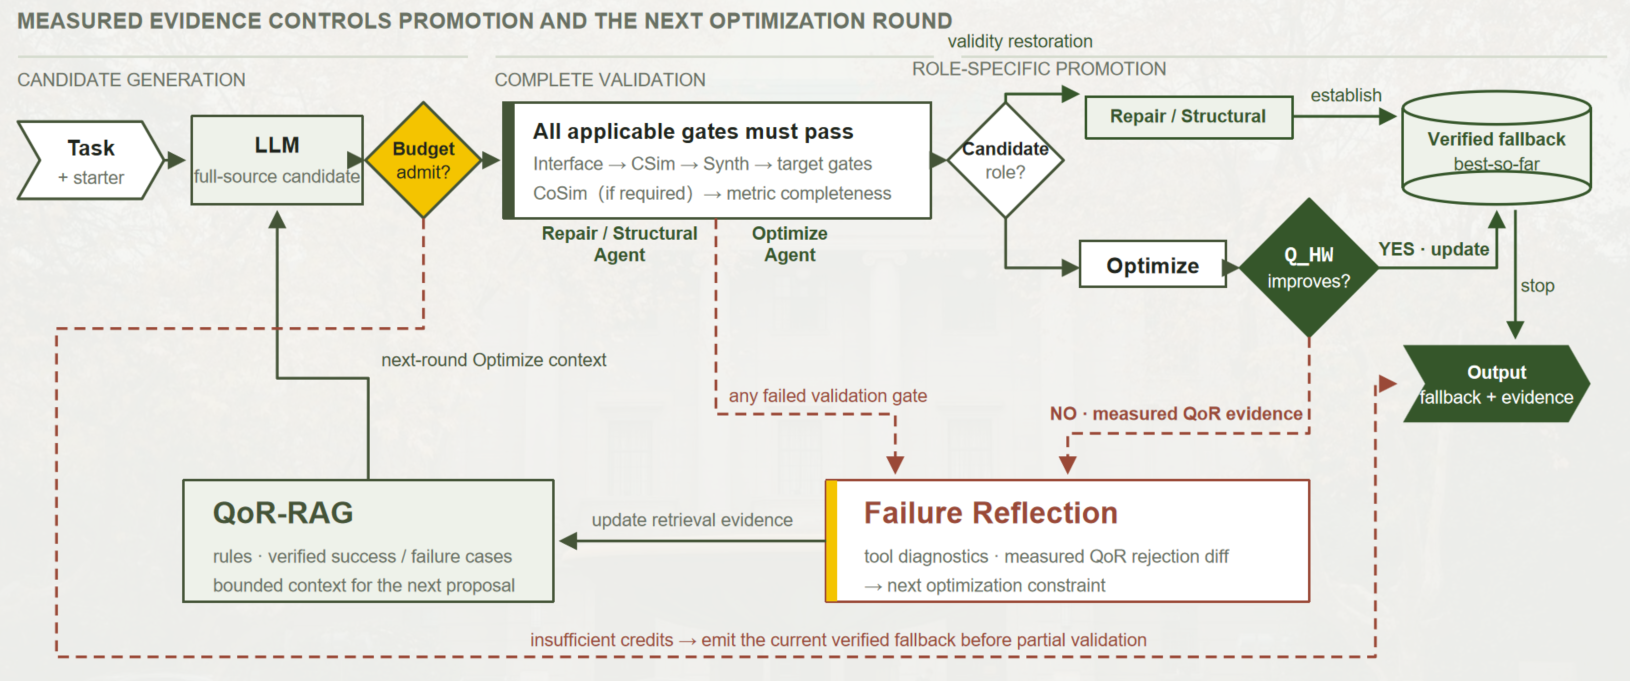
\includegraphics[width=\textwidth]{fig_vcl.png}
  \caption{\textbf{已验证候选回路。}
  候选方案仅在通过所有适用门且 $Q_{\mathrm{HW}}$ 提升后方可替代已验证备选。
  失败反思将工具诊断信息转化为下一轮约束，无需额外模型调用。}
  \label{fig:vcl}
\end{figure*}
